%File: anonymous-submission-latex-2024.tex
\documentclass[letterpaper]{article} % DO NOT CHANGE THIS
\usepackage[submission]{aaai24}  % DO NOT CHANGE THIS
\usepackage{times}  % DO NOT CHANGE THIS
\usepackage{helvet}  % DO NOT CHANGE THIS
\usepackage{courier}  % DO NOT CHANGE THIS
\usepackage[hyphens]{url}  % DO NOT CHANGE THIS
\usepackage{graphicx} % DO NOT CHANGE THIS
\urlstyle{rm} % DO NOT CHANGE THIS
\def\UrlFont{\rm}  % DO NOT CHANGE THIS
\usepackage{natbib}  % DO NOT CHANGE THIS AND DO NOT ADD ANY OPTIONS TO IT
\usepackage{caption} % DO NOT CHANGE THIS AND DO NOT ADD ANY OPTIONS TO IT
\frenchspacing  % DO NOT CHANGE THIS
\setlength{\pdfpagewidth}{8.5in} % DO NOT CHANGE THIS
\setlength{\pdfpageheight}{11in} % DO NOT CHANGE THIS
%
% These are recommended to typeset algorithms but not required. See the subsubsection on algorithms. Remove them if you don't have algorithms in your paper.
\usepackage{algorithm}
\usepackage{algpseudocode}

%New Package
\usepackage{tablefootnote}
\usepackage{mathtools}
\usepackage{amsfonts}
\usepackage{multirow}
\usepackage{multicol}
\usepackage{booktabs}
\usepackage[dvipsnames]{xcolor}
\usepackage{adjustbox}
\usepackage{makecell}

%
% These are are recommended to typeset listings but not required. See the subsubsection on listing. Remove this block if you don't have listings in your paper.
\usepackage{newfloat}
\usepackage{listings}
\DeclareCaptionStyle{ruled}{labelfont=normalfont,labelsep=colon,strut=off} % DO NOT CHANGE THIS
\lstset{%
	basicstyle={\footnotesize\ttfamily},% footnotesize acceptable for monospace
	numbers=left,numberstyle=\footnotesize,xleftmargin=2em,% show line numbers, remove this entire line if you don't want the numbers.
	aboveskip=0pt,belowskip=0pt,%
	showstringspaces=false,tabsize=2,breaklines=true}
\floatstyle{ruled}
\newfloat{listing}{tb}{lst}{}
\floatname{listing}{Listing}
%
% Keep the \pdfinfo as shown here. There's no need
% for you to add the /Title and /Author tags.
\pdfinfo{
/TemplateVersion (2024.1)
}

% DISALLOWED PACKAGES
% \usepackage{authblk} -- This package is specifically forbidden
% \usepackage{balance} -- This package is specifically forbidden
% \usepackage{color (if used in text)
% \usepackage{CJK} -- This package is specifically forbidden
% \usepackage{float} -- This package is specifically forbidden
% \usepackage{flushend} -- This package is specifically forbidden
% \usepackage{fontenc} -- This package is specifically forbidden
% \usepackage{fullpage} -- This package is specifically forbidden
% \usepackage{geometry} -- This package is specifically forbidden
% \usepackage{grffile} -- This package is specifically forbidden
% \usepackage{hyperref} -- This package is specifically forbidden
% \usepackage{navigator} -- This package is specifically forbidden
% (or any other package that embeds links such as navigator or hyperref)
% \indentfirst} -- This package is specifically forbidden
% \layout} -- This package is specifically forbidden
% \multicol} -- This package is specifically forbidden
% \nameref} -- This package is specifically forbidden
% \usepackage{savetrees} -- This package is specifically forbidden
% \usepackage{setspace} -- This package is specifically forbidden
% \usepackage{stfloats} -- This package is specifically forbidden
% \usepackage{tabu} -- This package is specifically forbidden
% \usepackage{titlesec} -- This package is specifically forbidden
% \usepackage{tocbibind} -- This package is specifically forbidden
% \usepackage{ulem} -- This package is specifically forbidden
% \usepackage{wrapfig} -- This package is specifically forbidden
% DISALLOWED COMMANDS
% \nocopyright -- Your paper will not be published if you use this command
% \addtolength -- This command may not be used
% \balance -- This command may not be used
% \baselinestretch -- Your paper will not be published if you use this command
% \clearpage -- No page breaks of any kind may be used for the final version of your paper
% \columnsep -- This command may not be used
% \newpage -- No page breaks of any kind may be used for the final version of your paper
% \pagebreak -- No page breaks of any kind may be used for the final version of your paperr
% \pagestyle -- This command may not be used
% \tiny -- This is not an acceptable font size.
% \vspace{- -- No negative value may be used in proximity of a caption, figure, table, section, subsection, subsubsection, or reference
% \vskip{- -- No negative value may be used to alter spacing above or below a caption, figure, table, section, subsection, subsubsection, or reference

\setcounter{secnumdepth}{0} %May be changed to 1 or 2 if section numbers are desired.

% The file aaai24.sty is the style file for AAAI Press
% proceedings, working notes, and technical reports.
%

% Title

% Your title must be in mixed case, not sentence case.
% That means all verbs (including short verbs like be, is, using,and go),
% nouns, adverbs, adjectives should be capitalized, including both words in hyphenated terms, while
% articles, conjunctions, and prepositions are lower case unless they
% directly follow a colon or long dash
\title{Social Influence Learning for Recommendation Systems}
\author{
    %Authors
    % All authors must be in the same font size and format.
    Written by AAAI Press Staff\textsuperscript{\rm 1}\thanks{With help from the AAAI Publications Committee.}\\
    AAAI Style Contributions by Pater Patel Schneider,
    Sunil Issar,\\
    J. Scott Penberthy,
    George Ferguson,
    Hans Guesgen,
    Francisco Cruz\equalcontrib,
    Marc Pujol-Gonzalez\equalcontrib
}
\affiliations{
    %Afiliations
    \textsuperscript{\rm 1}Association for the Advancement of Artificial Intelligence\\
    % If you have multiple authors and multiple affiliations
    % use superscripts in text and roman font to identify them.
    % For example,

    % Sunil Issar\textsuperscript{\rm 2},
    % J. Scott Penberthy\textsuperscript{\rm 3},
    % George Ferguson\textsuperscript{\rm 4},
    % Hans Guesgen\textsuperscript{\rm 5}
    % Note that the comma should be placed after the superscript

    1900 Embarcadero Road, Suite 101\\
    Palo Alto, California 94303-3310 USA\\
    % email address must be in roman text type, not monospace or sans serif
    proceedings-questions@aaai.org
%
% See more examples next
}

%Example, Single Author, ->> remove \iffalse,\fi and place them surrounding AAAI title to use it
\iffalse
\title{My Publication Title --- Single Author}
\author {
    Author Name
}
\affiliations{
    Affiliation\\
    Affiliation Line 2\\
    name@example.com
}
\fi

\iffalse
%Example, Multiple Authors, ->> remove \iffalse,\fi and place them surrounding AAAI title to use it
\title{My Publication Title --- Multiple Authors}
\author {
    % Authors
    First Author Name\textsuperscript{\rm 1},
    Second Author Name\textsuperscript{\rm 2},
    Third Author Name\textsuperscript{\rm 1}
}
\affiliations {
    % Affiliations
    \textsuperscript{\rm 1}Affiliation 1\\
    \textsuperscript{\rm 2}Affiliation 2\\
    firstAuthor@affiliation1.com, secondAuthor@affilation2.com, thirdAuthor@affiliation1.com 
}
\fi


% REMOVE THIS: bibentry
% This is only needed to show inline citations in the guidelines document. You should not need it and can safely delete it.
\usepackage{bibentry}
% END REMOVE bibentry

\begin{document}

\maketitle

\begin{abstract}
Social recommendation systems leverage the social relations among users to deal with the inherent cold-start problem in user-item interactions. However, previous models only treat the social graph as the static auxiliary to the user-item interaction graph, rather than dig out the hidden essentials and optimize them for better recommendations. Thus, the potential of social influence is still under-explored. In this paper, we will fill this gap by proposing a novel model for social influence learning to derive the essential influence patterns within the user relationships. Our model views the social influence from the perspectives of (1) the diversity of neighborhood's influence on the users, (2) the disentanglement of neighborhood's influence on the users, and (3) the exploration of underlying implicit social influence. To this end, we first employ a novel layerwise graph-enhanced variational autoencoder for the reconstruction of neighborhoods' representations, which aims to learn the pattern of social influence as well as simulate the social profile of each user for overcoming the sparsity issue in social relation data. Meanwhile, we introduce a layerwise graph attentive network for capturing the most influential scope of neighborhood. Finally, we adopt a dual sampling process to generate new social relations for enhancing the social recommendation. Extensive experiments have been conducted on three widely-used benchmark datasets, verifying the superiority of our model compared with state-of-the-art approaches.
\end{abstract}

% \begin{abstract}
% Social recommendation systems try to leverage the social relations among users to deal with the inherent cold-start problem in user-item interactions. However, previous models can only treat the social relation data as the static auxiliary to the user-item interaction data, rather than dig out the hidden essentials and optimize them for a better recommendation. Thus, the potential of social influence is still under-explored. In this paper, we will fill this gap by proposing a novel model for social influence learning to derive the essentail influence patterns in the user relationships. This model views the social influence from the perspectives of (1) the influence disentanglement of users on their neighborhood; (2) the influence diversity of users' neighborhoods; and (3) the potential exploration of implicit social influence. To this end, we first introduce a layerwise graph attentive network for capturing the most influential layers of neighborhoods. Meanwhile, a layerwise graph-enhanced variational graph autoencoder is employed for the reconstruction of neighborhoods' representation, which is considered to learn the pattern of social influence as well as simulate the social profile of each user for overcoming the sparsity of social relation data. Finally, we adopt dual sampling process that generate new social relations to enhance the social recommendation. Extensive experiments have been conducted on three widely-used benchmark datasets, verifying the superiority of our model compared with state-of-the-art approaches.
% \end{abstract}

\section{Introuduction}
%Due to the proliferation of the Internet, information overload is becoming a severe problem for human beings. Consequentially, both decision deficiency and the issue of personalization are also troublesome. To alleviate them, recommendation systems are designed to help people discover new products, services, and content that we might be keen on but not have found yet. One of the most fundamental methods is Collaborative Filtering (CF) \cite{using_cf, empirical_analysis}. It is based on the naive premise that similar user behaviors can be utilized to predict potential items. However, CF is affected by the various inherent vices (e.g. sparsity, cold-start, long tail problem) \cite{toward_next_generation}. By treating the user-item interactions as a matrix, both users and items are transferred into low dimensional latent matrices, which empower strong generalization ability to improve recommendations \cite{mf}. The user/item embeddings are usually generated by Singular Value Decomposition (SVD). Nowadays, with the bloom of deep learning, deep neural networks (DNNs) based recommendation system emerges. As one of the earliest DNN models for recommendations, NCF \cite{ncf} combines the Multilayer Perceptron (MLP) with user/item embeddings for training. A loss function guides the predicted ratings approximating the ground truth. Recently, graph neural networks (GNNs) show great achievement in a wide range of areas. By taking the user-item interactions into topological structure, GNN-based models aggregate the features from connected neighbors and cluster users as well as items by their associations \cite{ngcf}.\\
Social recommendation is a type of recommendation systems that leverages the social network among users to extract personalized information on individuals. According to the study of homophily in social networks \cite{birds_of_feather, dual_graph}, recommendation systems can be modeled not only based on users' purchase records but also their social relations. As commonly known, people may make decisions under the influence of their relatives. This is the so-called \textit{social influence}. Regarding the types of social influence, it is worth noting that \textit{explicit social influence} should be direct, trustworthy, and acknowledged connections among users, while \textit{implicit social influence} is the potential connections between users having similar preferences. In most scenarios, \textit{explicit social influence} can be retrieved from the relational data on social media. Previous works \cite{sorec, socialmf, trustsvd} have shown the outperformance of social recommendation systems as compared to general recommendation systems.

% The social recommendation is a specific type of recommendation systems that leverages the power of social networks of users, to provide personalized information to individuals. According to the study of homophily in social networks \cite{birds_of_feather, dual_graph}, not only can users receive recommendations based on their purchase records but their social relations as well. It has been convinced that people may make decisions under what they perceive from their relatives or friends, which is so-called \textit{social influence}. Regarding the types of social influence, it is worth noting that \textit{explicit social influence} should be direct, trustworthy, and acknowledged connections among users, while \textit{implicit social influence} is potential connections between users having similar preferences. In most scenarios, \textit{explicit social influence} can be retrieved from the relational data on social media. Previous works \cite{sorec, socialmf, trustsvd} have shown greater performance brought by social recommendation models compared with general recommendation systems.

While social recommendation has the capability to deal with personalization and correlations, there are still many challenges to address. Existing models mostly take the social relation data as the static auxiliary to the user-item interaction data, and they simply combine the data to handle the cold-start problem in recommendation. However, the shallow links given by the social relations may not reveal the essential influences among users. This problem is totally ignored by those previous works.
%Upon this paradigm, the unique characteristics and restrictions of social networks have been neglected. 
Overall, the following three challenges need to be attached importance:
% While social recommendation has the capability to deal with personalization and relevancy, there are still many challenges need to be addressed. Existing models mostly take the social relation data as the static auxiliary to the user-item interaction data, and simply combine them together for overcoming the cold-start problem. However, the shallow links given by the social relations may not reveal the esseintial influences among users. This problem is totally ignored by those previous works.
% %Upon this paradigm, the unique characteristics and restrictions of social networks have been neglected. 
% As shown in Figure \ref{fig_motivation}, we sort out and contend the following challenges that need to be attached importance.

\textit{Explicit Influence \uppercase\expandafter{\romannumeral 1} - Social Influence Diversity}: Users may connect with each other through various relationships (e.g. friends, family, and fellows, as shown in Figure 1(a)). Different types of relationships should have different patterns of influence passing. However, owing to the privacy issues, researchers face a lack of labels on relationships. Therefore, designing a fine-drawn model to disentangle the relationships is a de facto challenge. It is commonly believed that users of the same relationships should exhibit similar behaviors. In that case, we can simply cluster socially connected users that have bought the same items, and assign them with the same pseudo-relational labels. Nevertheless, users' social behaviors are much more elusive than we thought. The inconsistency and incompleteness of the original social network, conceived as social influence diversity, ought to be resolved on an ad hoc basis.

\textit{Explicit Influence \uppercase\expandafter{\romannumeral 2} - Social Influence Propagation}: Within the social network, users are interconnected as a whole. Under the scheme of GNN-based models, users can aggregate from a larger fraction of users that are not even directly connected. The challenge of social influence propagation is that different magnitudes of social influence exist on the graph. Moreover, users in closer neighborhoods may not always have higher social influence. Apart from local social influence that usually occurs in nearby neighborhoods (as shown in Figure 1(b)), global social influence from larger neighborhoods is also nonnegligible. Hence, instead of the proximity on graph, the magnitude of social influence propagation should depend on the consistency of behavior between the user and the neighborhoods, with higher consistency implying stronger social influence.

\textit{Implicit Influence - Social Influence Exploration}: Social influence is introduced to enhance the recommendation since it mitigates the data sparsity problem of user-item interactions. However, unlike user-item interactions, social influence is weak-tie relations, making it treacherous to be used to predict the strong-tie relations on the interaction graph. This impels us to work the other way round --- that is, to discover connections within the social network using the interaction graph. Through user-item interactions, users are thought to be making implicit influences on those who have bought similar items (as Figure 1(c)). This makes them potential neighbors on the social network. However, simply connecting these users on the social network is irrational and could cause user representation collapse. Moreover, it is a chicken and egg problem to determine the social network together with user representations.

To address these challenges, we propose \textbf{E}xplicit and \textbf{I}mplicit \textbf{I}nfluential \textbf{S}ocial \textbf{R}ecommendation \textbf{S}ystem (EIISRS). EIISRS consists of three corresponding stages: layerwise graph-enhanced variational autoencoder, layerwise graph attention networks, and dual sampling process. Our model is a two-tower training architecture, which includes a social path and a bipartite path. The social network and the user-item interaction graph are separately feed-forward to train two different types of user representations. This allows the model to automatically balance between two paths and avoid data entanglement. To perform social influence learning, we first apply Graph Convolutional Networks (GCN) to generate social user representations. Unlike the previous works, we take the social user representations generated from different layers of convolution for the training, so that we can model different scope of neighborhood separately and disentangle social influence. Next, the representation of each layer is fed into different VAEs to learn the distribution of neighborhoods, which contains the social patterns. Meanwhile, to simulate the social influence diversity, the reparameterization trick is used to sample neighborhood representations. The representations of different layers are then fused by a layerwise graph attention network for modeling the different magnitudes of social influence. Finally, to generate augmented neighborhoods for social influence exploration, a dual sampling (Gumbel sampling followed by Bernoulli sampling) is applied to prevent user representation collapse. Overall, the major contributions of this paper are summarized as follows:

\begin{itemize}
    \item We analyze and sort out three different challenges in social recommendation systems, and propose three novel components to deal with them accordingly.
    \item We propose a GCN-based two-tower architecture to incorporate a layerwise graph-enhanced variational autoencoder, a layerwise graph attention network, and a dual sampling process. To the best of our knowledge, we are the first to combine these methods for social network disentanglement in social recommendation systems. 
    \item We conduct extensive experiments on multiple real-world datasets to demonstrate the superiority of the proposed model and the effectiveness of each component. 
    % Technical appendix is attached at the end for detailed information. 
\end{itemize}

\begin{figure}[ht!]
  \centering
  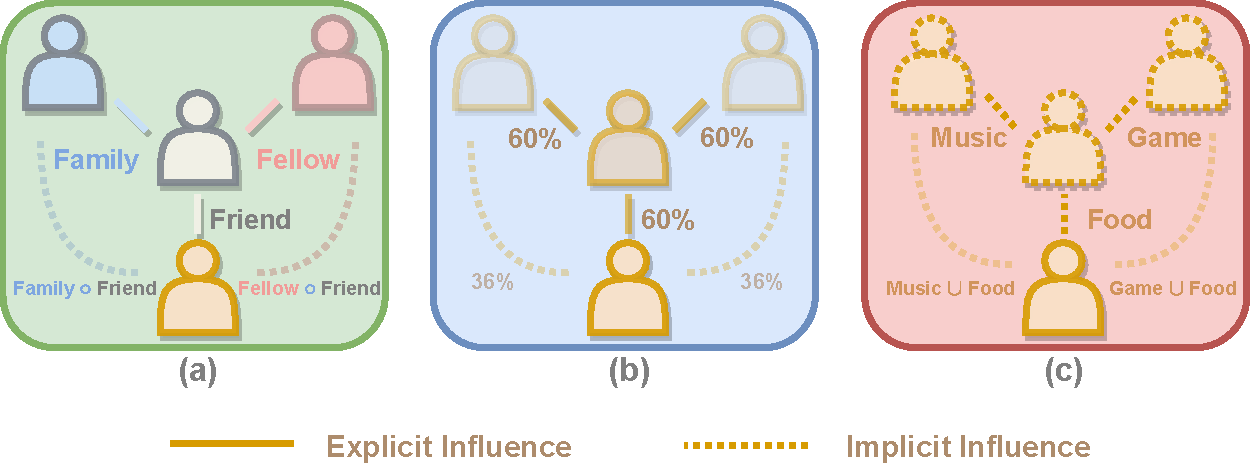
\includegraphics[width=0.451\textwidth]{motivation.pdf} %1.png是图片文件的相对路径
  \caption{Toy example of (a) Social Influence Diversity, (b) Social Influence Propagation, and (c) Social Influence Exploration.}
  \label{fig_motivation}
\end{figure}

\section{Methodology}
\begin{figure*}[ht]
  \centering
  \includegraphics[width=1.1\textwidth]{framework_all.pdf}
  \caption{The framework of the EIISRS.}
  \label{framework_all.pdf}
\end{figure*}

In this section, we introduce our model \textbf{EIISRS} in detail. We will elaborate on our framework and the three main components used to address the respective challenges of social influence modeling.

\subsection{Preliminaries}
Let $u$ denote the user and $i$ denote the item within the dataset. $\mathcal{U}=\{u_1,  u_2, \ldots, u_m\}$ represents the entire user set and $\mathcal{I}=\{i_1, i_2, \ldots, i_n\}$ represents the entire item set, where the total numbers of users and items are $|\mathcal{U}|=m$ and $|\mathcal{I}|=n$, respectively. $\textbf{\textit{R}} \in \mathbb{R}^{m\times n}$ is the binary user-item interaction matrix. Given a user-item pair $(u, i)$, $r_{u,i}=1$ implies that user $u$ purchased item $i$ and should be interested in it, whereas $r_{u,i}=0$ implies no interactions. $\textbf{\textit{S}} \in \mathbb{R}^{m\times m}$ refers to the social matrix, whose entries are $1$ if the corresponding users are socially connected and $0$ otherwise. We build a bipartite graph $\mathcal{G}_r=\{(u, r_{u,i}, i)|u\in \mathcal{U}, i\in \mathcal{I}, r_{u,i}\in \{0,1\}\}$ from the user-item interaction matrix $\textbf{\textit{R}}$. Similarly, we build a social graph $\mathcal{G}_s$ from the social matrix $\textbf{\textit{S}}$. $\mathcal{I}(u)$ is the item set containing the items purchased by user $u$. $\mathcal{N}(u)$ is the set of neighboring users who are directly connected to user $u$ on the social network. Each convolution layer in our model generates neighborhood representations. These representations are denoted as $\{\textbf{\textit{P}}^{(0)}, \textbf{\textit{P}}^{(1)}, \ldots, \textbf{\textit{P}}^{(L)}\}$ for users and $\{\textbf{\textit{Q}}^{(0)}, \textbf{\textit{Q}}^{(1)}, \ldots, \textbf{\textit{Q}}^{(L)}\}$ for items, where $\textbf{\textit{P}}^{(l)} \in \mathbb{R}^{m\times d}$ and $\textbf{\textit{Q}}^{(l)} \in \mathbb{R}^{n\times d}$ represent the $l$-th layer embeddings of $d$-dimensional size. In our model, we focus on top-K recommendations, and $\hat{r}_{u, i}$ denotes the computed likelihood that user $u$ is interested in item $i$, i.e., the recommendation score. In this paper, we use bold capital letters to denote matrices and bold lowercase letters to denote vectors.

% \subsection{Preliminaries}
% Let $u$ denote the user and $i$ denote the item recorded in the dataset. Then, we have $\mathcal{U}=\{u_1,  u_2, \ldots, u_m\}$ to denote the whole user set and $\mathcal{I}=\{i_1, i_2, \ldots, i_n\}$ the whole item set, where the total numbers of them are $|\mathcal{U}|=m$ and $|\mathcal{I}|=n$, respectively. $\mathcal{I}(u)$ is the itemset in which items purchased by user $u$ are included. $\mathcal{N}(u)$ is the set of neighbor users who are directly connected with user $u$ on the social networks. $\textbf{\textit{R}} \in \mathbb{R}^{m\times n}$ is the binary user-item interaction matrix. Suppose there is a pair $(u, i)$, $r_{u,i}=1$ implies that user $u$ purchased item $i$ and should be interested in it, whereas $r_{u,i}=0$ suggests that item $i$ is unknown to user $u$ or she is unconcerned about it. In our model, we concentrate on top-K recommendations, and $\hat{r}_{u, i}$ denotes the likelihood of item $i$ being recommended to user $u$. In terms of social networks, $\textbf{\textit{S}} \in \mathbb{R}^{m\times m}$ refers to the social matrix. It could be symmetric or asymmetric depending on whether the dataset is directional or not. Each convolution layer in our model would generate corresponding neighborhood representations, referring to $\{\textbf{\textit{P}}^{(0)}, \textbf{\textit{P}}^{(1)}, \ldots, \textbf{\textit{P}}^{(l)}\} \in \mathbb{R}^{m\times d}$ and $\{\textbf{\textit{Q}}^{(0)}, \textbf{\textit{Q}}^{(1)}, \ldots, \textbf{\textit{Q}}^{(l)}\} \in \mathbb{R}^{n\times d}$ as the user and item embeddings of $d$-dimensional size, respectively. In this paper, we use bold capital letters to denote matrices and lowercase letters to denote vectors. We build a bipartite graph $\mathcal{G}_r=\{(u, r_{u,i}, i)|u\in \mathcal{U}, i\in \mathcal{I}, r_{u,i}\in \{0,1\}\}$ from user-item interactions, and social graph $\mathcal{G}_s$ from relational matrix in the same way.

\subsection{Dual-Path Graph Convolution}
% In our model, we use a two-tower setting, including the bipartite path and the social path. The path that takes the bipartite graph as input is responsible for jointly encoding user representations and item representations, while the other is for encoding another user representation of explicit social influence. It is apparent to realize that different patterns on different graphs exhibit different importance to the performance of the final recommendation. Therefore, it is necessary to feed the base user representation $\textbf{\textit{P}}^{(0)}$ with partial masking to different paths. To control how much information is to feed forward, we introduce a preprocessing filter Self-Gating Units(SGUs) \cite{SGU}, which adopts the idea called multiplicative skip connection:
In our model, we use a two-tower setting, including the bipartite path and the social path. The bipartite path takes $\mathcal{G}_r$ as input and jointly encodes user and item representations. The social path takes $\mathcal{G}_s$ as input and encodes another set of user representations. Since the patterns on different graphs are of different importance to the representation learning, we need to control how much information to feed forward in each path. To achieve that, we propose to preprocess the base user representations $\textbf{\textit{P}}^{(0)}$ with dual partial maskings, which can be learned using the filtering Self-Gating Units (SGUs) \cite{SGU} that adopt the idea called multiplicative skip connection:
\begin{equation}
    \textbf{\textit{P}}^{(0)}_{path} = f_{sgu}(\textbf{\textit{P}}^{(0)}) = \textbf{\textit{P}}^{(0)} \odot \sigma (\textbf{\textit{P}}^{(0)}\textbf{\textit{W}}^{path} + \textbf{\textit{b}}^{path}),
\end{equation}
where $\textbf{\textit{W}}^{path} \in \mathbb{R}^{d\times d}$ and $\textbf{\textit{b}}^{path} \in \mathbb{R}^{d}$ are learnable parameters, $path \in \{r,s\}$ denotes the path, $\odot$ represents the Hadamard product, and $\sigma$ is the nonlinear activation function. Here we use the sigmoid function as the activation since it squashes the values into $[0,1]$ for the gating.

Referring to the graph convolutional scheme proposed in \cite{GCN}, graph convolutions in our model can be rewritten as:
\begin{gather}
    \textbf{\textit{P}}^{(l+1)}_{r} = \textbf{\textit{D}}^{-1}_{user}\textbf{\textit{R}}\textbf{\textit{Q}}^{(l)},\\
    \textbf{\textit{Q}}^{(l+1)} = \textbf{\textit{D}}^{-1}_{item}\textbf{\textit{R}}^{\top}\textbf{\textit{P}}^{(l)}_{r},\\
    \textbf{\textit{P}}^{(l+1)}_{s} = \textbf{\textit{D}}^{-1}_{s}\textbf{\textit{S}}\textbf{\textit{P}}^{(l)}_{s},
\end{gather}
where $\textbf{\textit{P}}^{(l)}_{r}$ and $\textbf{\textit{P}}^{(l)}_{s}$ are the $l$-th layer user representations generated from the user-item interaction graph and social graph, respectively. $\textbf{\textit{D}}_{user}$, $\textbf{\textit{D}}_{item}$, and $\textbf{\textit{D}}_{s}$ are the diagonal degree matrices of $\textbf{\textit{R}}$, $\textbf{\textit{R}}^{\top}$, and $\textbf{\textit{S}}$. We follow the guidance of LightGCN \cite{lightgcn} and employ neighborhood information aggregations without feature transformations and nonlinear activation function. 
% It is proven to be effective and efficient for recommendations.

\subsection{Social Influence Learning}
After the elementary graph convolutions, the social influence learning phase follows to capture comprehensive social patterns for improved recommendations.
\subsubsection{Social Influence Diversity.}
Social influence is diverse as users are interconnected over various relationships. Moreover, social networks are sparse. Only part of the links are observable while the rest remain unknown. Therefore, one way to optimize social network modeling is to apply link predictions and abnormal detections. However, it will be expensive to train such a model, and the model will need to comply with a pre-training/fine-tuning framework. We wish to use a lightweight and end-to-end scheme for capturing the social influence diversity. 

To this end, we use VAE \cite{VAE} as a building block and propose Layerwise Graph-Enhanced Variational AutoEncoder (LGE-VAE). Specifically, the input features of LGE-VAE are $\{\textbf{\textit{P}}^{(0)}_{s}, \textbf{\textit{P}}^{(1)}_{s}, \ldots, \textbf{\textit{P}}^{(L)}_{s}\}$, the layerwise neighborhood representations learned from previous social graph convolutions. LGE-VAE encodes these features as layerwise distributions over the latent space. Then, LGE-VAE samples a set of representations $\{\textbf{\textit{Z}}_s^{(0)}, \textbf{\textit{Z}}_s^{(1)}, \ldots, \textbf{\textit{Z}}_s^{(L)}\}$ for each user from the layerwise distributions. The uncertainty within the sampling process helps to capture the diversity in social influence. Finally, a decoder is used to reconstruct the input features. 

Overall, the encoder can be viewed as the posterior distribution $p_{\phi}(\textbf{\textit{Z}}_s^{(l)}|\textbf{\textit{P}}_s^{(l)})$ with learnable parameters $\phi$. Following the conventions, the intractable posterior distribution is approximated with a Gaussian distribution as the prior distribution, defined as follows:
% Social influence are diverse. The existing social links are not enough to directly reflect an overall preference among items. More importantly, social networks are sparse, and only part of them is observable while the rest remain unknown. Therefore, social networks had better be optimized with link prediction and abnormal detection. However, it will spend extraordinary resources training the model for social networks, and the model needs to comply with the pre-training/fine-tuning process in this way. We hope for a lightweight end-to-end model, focusing on our main task of recommendation. To this end, we use the VAE \cite{VAE} as a building block, and present Layerwise Graph-Enhanced Variational AutoEncoder (LGE-VAE). As a generative model, LGE-VAE generates a set of new sampled representations for each user, which is comprised of information about the neighborhood in certain layers. Concretely, LGE-VAE is followed with graph convolution, learning the distribution of social influence from neighbors' representation in the range of designated layers. The encoders take the representation as features and encode them into latent representations that better depict the general social pattern. And then the decoder reconstructs the original neighborhood representation derived from the plain graph structure. The encoder can be seen as the posterior distribution $p_{\phi}(\textbf{\textit{z}}|\textbf{\textit{P}}_s^{(l)})$ with learnable parameters $\phi$. We keep the common manner that approximates the intractable posterior distribution with Gaussian distribution as the prior distribution, defined as:
\begin{align}
    q_{\phi}(\textbf{\textit{Z}}_s^{(l)}|\textbf{\textit{P}}_s^{(l)}) = \mathcal{N}(\mu(\textbf{\textit{P}}_s^{(l)}), \sigma^2(\textbf{\textit{P}}_s^{(l)})),
\end{align}
where $\mu(\cdot)$ and $\sigma(\cdot)$ are the functions that compute the mean and standard deviation for the layerwise representations. Here, we assume that the Gaussian distribution is anisotropic. That is, the deviations of layerwise neighborhood distributions are different across users and dimensions. This helps to capture each user's unique interests and affection to items \cite{ESRF}. 

Specifically, the encoder of LGE-VAE generates the layerwise mean $\boldsymbol{\mu}^{(l)} \in \mathbb{R}^{m\times d}$ and the layerwise standard deviation $\boldsymbol{\sigma}^{(l)} \in \mathbb{R}^{m\times d}$. Given the distributions, we apply the reparameterization trick to sample new social neighborhood representations:
\begin{gather}
    \boldsymbol{\mu}^{(l)}, \boldsymbol{\sigma}^{(l)} = MLP(\textbf{\textit{P}}_{s}^{(l)}, \textbf{\textit{W}}_{enc}),\\
    \textbf{\textit{Z}}_s^{(l)} = \boldsymbol{\mu}^{(l)}+\boldsymbol{\sigma}^{(l)}\odot\boldsymbol{\epsilon}, \boldsymbol{\epsilon} \sim \mathcal{N}(0,\textbf{I}),
\end{gather}
where $\textbf{\textit{W}}_{enc} \in \mathbb{R}^{m\times d}$ is the learnable parameter for the encoder, $MLP(\cdot): \mathbb{R}^{m\times d}\times \mathbb{R}^{d\times d} \mapsto \mathbb{R}^{m\times d}$ is the Multilayer Perceptron (MLP), and $\boldsymbol{\epsilon} \in \mathbb{R}^{m\times d}$ is the Gaussian noise. This sampling process can be regarded as a simulation of social influence diversity. Then, we take the negation of the Evidence Lower Bound (ELBO) as the loss function of LGE-VAE, which is defined as follows:
\begin{equation}
    \begin{split}
        \mathcal{L}_{vae}(\psi,\phi,\beta)=
        &-\mathbb{E}_{q_\phi}[\log p_{\psi}(\textbf{\textit{P}}_s^{(l)}|\textbf{\textit{Z}}_s^{(l)})]\\
        &+\beta KL (q_{\phi}(\textbf{\textit{Z}}_s^{(l)} | \textbf{\textit{P}}_s^{(l)}) || p(\textbf{\textit{Z}}_s^{(l)})),
    \end{split}
\end{equation}
where $\phi$ and $\psi$ are learnable parameters of the encoder and decoder, respectively. The first term is the reconstruction loss while the second term is the KL divergence loss. Here we adopt $\beta$-VAE, where the hyperparameter $\beta$ helps to discover disentangled latent factors. When $\beta \rightarrow 1$, $\beta$-VAE degrades to regular VAE, in which the KL divergence will take as much importance as the reconstruction loss. We set $\beta \ll 1$ to prioritize the reconstruction loss and stabilize the training of the encoder. It is worth noting that, LGE-VAE is different from VAE and VGAE in that it inputs neither the real-world attributes as features nor the entire graph structure.

\subsubsection{Social Influence Propagation.}
The previous graph convolutions and social diversity simulations together generate a set of representations $\{\textbf{\textit{Z}}_s^{(0)}, \textbf{\textit{Z}}_s^{(1)}, \ldots, \textbf{\textit{Z}}_s^{(L)}\}$ for each user, where $\textbf{\textit{Z}}_s^{(l)}$ contains the social influence within the $l$-hop neighborhood. The question that follows immediately is how to aggregate these multilayer social representations. As shown in Table \ref{table_agg}, there are four main categories of aggregation methods. For instance, mean pooling is the most commonly used one, which is proven to be effective in preventing over-smoothing. However, it cannot well disentangle the social influence of distinct layers. Meanwhile, social influence should be propagated from a neighborhood of appropriate size, neither too large that consists of noise nor too small that results in collapse. To this end, we apply the attention mechanism \cite{attention} to aggregate the layerwise social representations. For each user $u$, the tuple $(\boldsymbol{\alpha}_{0},\boldsymbol{\alpha}_{1},\ldots,\boldsymbol{\alpha}_{L})$ contains the attention scores for each layer of representations. The function to compute the attention scores is $f_{att}$, defined as:
% Social influence propagation takes effect simultaneously with social graph convolution. After propagation through $L$ layers, we use the attention mechanism \cite{attention} to aggregate the user social representation. As shown in Table \ref{table_agg}, there are four main categories of aggregation methods. Mean pooling is the most commonly used one. It is proven to avoid the over-smoothing problem. However, it cannot well disentangle the information over users' social influence. Users should be appealing to an appropriate size of neighborhoods, neither is so huge that consists of noise nor so tiny that results in collapse. Concerning each user $u$, a tuple $(\boldsymbol{\alpha}_{0},\boldsymbol{\alpha}_{1},\ldots,\boldsymbol{\alpha}_{L})$ contains the attention scores for measuring distinct contributions of layer $l$ to the final recommendation performance. The function to calculate the attention score is $f_{att}$, defined as:
% \begin{align}
%     \boldsymbol{\alpha}_l = f_{att}(\textbf{\textit{P}}_{s}^{(l)}) = \frac{\exp(\textbf{\textit{a}}^{\top}\textbf{\textit{W}}_{att} \textbf{\textit{P}}^{(l)}_{s})}{\sum_{j=0}^{L}\exp(\textbf{\textit{a}}^{\top}\textbf{\textit{W}}_{att}\textbf{\textit{P}}^{(j)}_s)},
% \end{align}
% where both $\textbf{\textit{a}}\in \mathbb{R}^{d}$ and $\textbf{\textit{W}}_{att}\in \mathbb{R}^{d\times d}$ are trainable parameters, and the final representation $\textbf{\textit{P}}_s=\sum_{l=0}^{L}{\boldsymbol{\alpha}_l\textbf{\textit{P}}^{(l)}_s}$. Practically, we use the sampled neighborhood representation $\textbf{\textit{z}}^{(l)}$ instead of $\textbf{\textit{P}}_s^{(l)}$.
\begin{align}
    \boldsymbol{\alpha}_l = f_{att}(\textbf{\textit{Z}}_{s}^{(l)}) = \frac{\exp(\textbf{\textit{a}}^{\top}\textbf{\textit{W}}_{att} \textbf{\textit{Z}}^{(l)}_{s})}{\sum_{j=0}^{L}\exp(\textbf{\textit{a}}^{\top}\textbf{\textit{W}}_{att}\textbf{\textit{Z}}^{(j)}_s)},
\end{align}
where both $\textbf{\textit{a}}\in \mathbb{R}^{d}$ and $\textbf{\textit{W}}_{att}\in \mathbb{R}^{d\times d}$ are trainable parameters. The final representation after the aggregation is $\widetilde{\textbf{\textit{P}}}_s=\sum_{l=0}^{L}{\boldsymbol{\alpha}_l\textbf{\textit{Z}}^{(l)}_s}$.

In fact, explicit social influence is usually very noisy. Even shallow (e.g., 1-hop) propagations can contain much noise, making it hard to extract useful information therefrom  \cite{noisy1,noisy2}. Recently, layerwise weighted graph network has shown effectiveness on graph representation learning \cite{GGSNN, MLAP}, but it has yet to find its place in recommendations. The LightGCN experiment \cite{lightgcn} demonstrated the futility of layerwise graph attention for recommendations, as the user-item bipartite graph does not reflect informative patterns between layers. Different from previous works, we are the first to apply layerwise attention mechanism for social recommendation tasks. It helps to balance layerwise messages and filter out noise on the social graph, such that useful information can be extracted despite the noisiness in explicit social influence. 
% It is worth noting that, explicit social influence usually is too noisy to bet on its effective indications even from lower layers \cite{noisy1,noisy2}. Attention mechanism can help balance the information and noise by layers, known as local influence from relatives and global influence from popularity. Layer-wise graph attention has shown its performance on learning graph representation \cite{GGSNN, MLAP}. However, LightGCN argues for its futility in recommendations by experiments, since the bipartite graph does not reflect such patterns. Different from the previous work, we are the first to make an attempt at social graph in recommendations, in the manner of explicit social influence.
\begin{table}[ht]\small
    \begin{tabular*}{\columnwidth}{@{\extracolsep{\fill}}c|c|c}
    \hline
    \centering
    \textbf{Method} & \textit{Agg($\cdot)$} & \textbf{Model}
    \\ \hline
        \hline
        \thead{Mean}            &$\frac{1}{L+1}\sum^{L}_{l=0}{\textbf{\textit{Z}}^{(l)}}$    &\thead{LightGCN\cite{lightgcn}}                                                  \\
        \thead{Max}              &${\underset{l}{\mathrm{max}}} (\textbf{\textit{Z}}^{(l)})$ &\thead{GCN\cite{GCN}}                                            \\
        \thead{Concat.}            &$\mathbin\Vert^{L}_{l=0}\textbf{\textit{Z}}^{(l)} $ &\thead{NGCF\cite{ngcf}}
            \\
        Att.              %&$Att(\textbf{\textit{P}}^{(0)}\ldots\textbf{\textit{P}}^{(L)})$ 
        &$\sum_{l=0}^{L}{\boldsymbol{\alpha}_l\textbf{\textit{Z}}^{(l)}}$
        &\thead{MLAP\cite{MLAP}}
            \\
        \hline
    \end{tabular*}
    \caption{Methods for aggregating layerwise representations.}
    \label{table_agg}
\end{table}

% \begin{table}[ht]\small
%     \centering
%     %\renewcommand{\arraystretch}{1.5} % Default value: 1
%     %\begin{adjustbox}{max width=8cm}
%     \begin{tabular}{c|c|c}
%     \hline
%     \textbf{Catagory} & \textit{Agg($\cdot)$} & \textbf{Model}
%     \\ \hline
%         \hline
%         \thead{Mean\\ Pooling}            &$\frac{1}{L}\sum^{L}_{l=0}{\textbf{\textit{P}}^{(l)}}$    &\thead{LightGCN\\ \cite{lightgcn}}                                                  \\
%         \thead{Max\\ Pooling}              &$\underset{l}{\mathrm{argmax}} (\textbf{\textit{P}}^{(l)})$ &\thead{MGNM\\ \cite{MGNM}}                                                 \\
%         \thead{Concat-\\enation}            &$\mathbin\Vert^{L}_{l=0}\textbf{\textit{P}}^{(l)} $ &\thead{NGCF\\ \cite{ngcf}}
%             \\
%         Attention               %&$Att(\textbf{\textit{P}}^{(0)}\ldots\textbf{\textit{P}}^{(L)})$ 
%         &$\sum_{l=0}^{L}{\boldsymbol{\alpha}_l\textbf{\textit{P}}^{(l)}}$
%         &\thead{MLAP\\ \cite{MLAP}}
%             \\
%         \hline
%     \end{tabular}
%     %\end{adjustbox}  
%     \caption{Different methods for aggregating the embeddings obtained in layers.}
%     \label{table_agg}
% \end{table}

\subsubsection{Social Influence Exploration.}
Apart from explicit social influence, implicit social influence also plays an important role in social recommendations, since it aligns the social graph with the user-item bipartite graph via indirect relations between users. Different from social diversity simulation that endeavors to improve representations, social influence exploration aims to model the connectivity between users on the social network. To this end, we adopt selector layers with Gumbel sampling \cite{gumbel,ESRF}, which simulates relation sampling under an extreme value distribution.
This generates a new list of candidate neighbors for each user based on top-$K$ relations. Formally, we apply $K$ selectors to compute the scores between users. For user $u$ and selector $i$, the scores between $u$ and other users are defined as follows:
\begin{gather}
    Sim(u, i) = act((\textbf{\textit{P}}_r \textbf{\textit{p}}_u^{\top})\odot \textbf{\textit{W}}_{select}^{(i)}),\\
    Score(u, i) = Softmax(\frac{\log(Sim(u, i)+\textbf{\textit{g}})}{\tau}),
\end{gather}
where $\textbf{\textit{P}}_{r}=\frac{1}{L+1}\sum_{l=0}^{L}{\textbf{\textit{P}}^{(l)}_r}$ and $\textbf{\textit{p}}_u \in \textbf{\textit{P}}_r$ is the representation of user $u$ in bipartite path. $\textbf{\textit{W}}_{select}^{(i)} \in \mathbb{R}^m$ is the learnable $i$-th selector. $act(\cdot)$ is the activation function. $\textbf{\textit{g}} \in \mathbb{R}^{m}$ is the Gumbel noise generated by $\textbf{\textit{g}}=-\log(-\log(\boldsymbol{\mu}))$, where $\boldsymbol{\mu} \sim \mathcal{N}(0,\textbf{I})$. $\tau$ is the temperature and the scores become discrete when $\tau \rightarrow 0$. Scores from all $K$ selectors are summed up to get the top-$K$ candidate neighbors.
% $Sim(\cdot)$ is a function that calculates the similarity between user $u$ and all other users and $\textbf{\textit{p}}_u \in \textbf{\textit{P}}_r$. $act(\cdot)$ is the nonlinear activation function.  is the learnable $i^{th}$ selector, where there are $K$ selectors in total. $\textbf{\textit{g}} \in \mathbb{R}^{m}$ is the Gumbel noise that generates from $\textbf{\textit{g}}=-\log(-\log(\boldsymbol{\mu}))$, where $\boldsymbol{\mu} \sim \mathcal{N}(0,\textbf{I})$. $\tau$ serves as the temperature and the scores become discrete when $\tau \rightarrow 0$.
% Apart from explicit social influence, many reasons impel us to activate recommendation systems with implicit social influence. One of the most important ones is to align social networks with indirect relations in bipartite interaction graphs. Noting that, different from social diversity simulation that endeavors to improve representations, social influence exploration concentrates on the connectivity of social networks in the primary stage. To this end, we adopt concrete selector layers with Gumbel sampling \cite{gumbel} for generating a new list of candidate neighbors for each user. Gumbel distribution is used to simulate the top-K proximate relations under the extremum distribution scheme. Formally, we set $s$ neurons as selectors in the MLPs, and calculate the scores among all users. For each selector, the score is defined as:
% \begin{gather}
%     Sim(\textbf{\textit{p}}_u,\textbf{\textit{P}}_r) = act((\textbf{\textit{P}}_r \textbf{\textit{p}}_u^{\top})\odot \textbf{\textit{W}}_{select}^{(i)}),\\
%     Score(i) = Softmax(\frac{\log(Sim(\cdot)+\textbf{\textit{g}})}{\tau}),
% \end{gather}
% where $Sim(\cdot)$ is a function that calculates the similarity between user $u$ and all other users and $\textbf{\textit{p}}_u \in \textbf{\textit{P}}_r$. $act(\cdot)$ is the nonlinear activation function. $\textbf{\textit{W}}_{select}^{(i)} \in \mathbb{R}^m$ is the learnable $i^{th}$ selector, where there are $K$ selectors in total. $\textbf{\textit{g}} \in \mathbb{R}^{m}$ is the Gumbel noise that generates from $\textbf{\textit{g}}=-\log(-\log(\boldsymbol{\mu}))$, where $\boldsymbol{\mu} \sim \mathcal{N}(0,\textbf{I})$. $\tau$ serves as the temperature and the scores become discrete when $\tau \rightarrow 0$.

However, directly connecting users with their $K$ candidate neighbors on the social network can damage the network architecture. If the candidate neighbors share highly similar preferences, it will harm the social influence diversity and cause user representation collapse \cite{collapse}. To retain the information entropy on graph, for each user $u$, we perform a follow-up Bernoulli sampling on the $|\mathcal{N}(u)|$ explicit neighbors and $K$ candidate neighbors as follows:
% However, straightforward insertions of social networks are likely to damage the architecture of our model and lead to a suboptimal result. The user representation collapse \cite{collapse} occurs when the numerous implicit neighbors with highly similar preferences deteriorate the interior diversity in social diversity simulation. Therefore, we introduce the follow-up Bernoulli distribution as dual sampling to retain the information entropy in social networks. In detail, the number of users we choose after selectors are correlated with the number of neighbors in the original social networks under the Bernoulli distribution:
\begin{gather}
    \widetilde{\mathcal{N}}(u) \sim Bernoulli(\frac{|\mathcal{N}(u)|}{K+|\mathcal{N}(u)|}),\\
    \widetilde{\textbf{\textit{S}}} = \mathbin\Vert_{u=0}^{m}\widetilde{\mathcal{N}}(u),
\end{gather}
where $\widetilde{\mathcal{N}}(u) \in \mathbb{R}^{m}$ denotes the new neighbor set of user $u$ and  $\widetilde{\textbf{\textit{S}}} \in \mathbb{R}^{m\times m}$ denotes the new social network. After dual sampling, the number of user $u$'s connected neighbors should be around $|\mathcal{N}(u)|$, the initial number of neighbors. We set $\widetilde{\textbf{\textit{S}}}=\textbf{\textit{S}}$ in the first epoch of training and update it in each following epoch with the dual sampling process. As the training phases proceed, the social graph keeps being reconstructed. It could be seen as graph augmentation to activate and learn the comprehensive social pattern. 
% where $|\mathcal{N}(u)| \in \mathbb{R}$ is the number of user $u$'s explicit social neighbors in the original data. $\widetilde{\mathcal{N}}(u) \in \mathbb{R}^{m}$ denotes the new neighbor set of user $u$ and  $\widetilde{\textbf{\textit{S}}} \in \mathbb{R}^{m\times m}$ denotes the new social network. We set $\widetilde{\textbf{\textit{S}}}=\textbf{\textit{S}}$ in the first epoch of training and update it using the dual sampling scheme in each epoch.
% . Specifically, for each user, the number of connected neighbors after dual sampling should be approximately the same as the number of explicit neighbors in the original data:

\subsection{Model Optimization}
Now that the user embeddings $\widetilde{\textbf{\textit{P}}}_{s}$ in the social path have gone through the social influence learning stage, they will be aggregated with the user embeddings $\textbf{\textit{P}}_{r}$ in the bipartite graph. Even though $\widetilde{\textbf{\textit{P}}}_{s}$ and $\textbf{\textit{P}}_{r}$ are both generated from the same initial embeddings, they do not exist in the same feature space because $\widetilde{\textbf{\textit{P}}}_{s}$ contains transformations from LGE-VAE. Consequently, $\widetilde{\textbf{\textit{P}}}_{s}$ may not be directly applied for item predictions on the user-item common space, i.e., the space shared by $\textbf{\textit{P}}_{r}$ and $\textbf{\textit{Q}}$. To obtain well-unified user embeddings, we transform $\widetilde{\textbf{\textit{P}}}_{s}$ before the aggregation:
% After user embeddings on the social path have gone through all these three components, they would be aggregated with user embeddings generated from the user-item interactions graph and we get the final embeddings of users. Even though the $\widetilde{\textbf{\textit{P}}}_{s}$ and $\textbf{\textit{P}}_{r}$ are generated from the same initial embeddings and settle in the same feature space, the proximity of users represented in the social path may not accurately reflect on desired items prediction. To obtain well-unified user embeddings, we assign an aggregation matrix to fix this problem:
\begin{align}
    \textbf{\textit{P}}_{final} = \textbf{\textit{P}}_{r} + act(\widetilde{\textbf{\textit{P}}}_{s}\textbf{\textit{W}}_{agg}),
\end{align}
where $\textbf{\textit{W}}_{agg} \in \mathbb{R}^{d\times d}$ is a learnable transformation matrix. To train the model, we use the pairwise Bayesian Personalized Ranking (BPR) \cite{bpr} as our recommendation loss function: 
\begin{align}
    \mathcal{L}_{rec} = \sum_{i\in \mathcal{I}(u), j\notin \mathcal{I}(u)}{-\log \sigma(\hat{r}_{u,i}(\boldsymbol{\Omega})-\hat{r}_{u,j}(\boldsymbol{\Omega}))},
\end{align}
where $\boldsymbol{\Omega}$ refers to all learnable parameters of our model. $\hat{r}_{u,i}$ is the predicted score for user $u$ on item $i$, where $\hat{r}_{u,i}=\textbf{\textit{p}}_u \textbf{\textit{q}}_i$, $\textbf{\textit{p}}_u \in \textbf{\textit{P}}_{final}$ and $\textbf{\textit{q}}_i \in \textbf{\textit{Q}}$. $\sigma(\cdot)$ is the sigmoid function. The L2 regularization is omitted for simplification. At last, we integrate the recommendation loss $\mathcal{L}_{rec}$ with the LGE-VAE loss $\mathcal{L}_{vae}$, which consists of the reconstruction loss and the KL divergence loss. Overall, the objective function of EIISRS is formulated as:
% We define the recommendation as the main task of training and thus we assign the coefficients to the others:
\begin{align}
    \mathcal{L}_{total} = \mathcal{L}_{rec} + \gamma\mathcal{L}_{vae},
\end{align}
where $\gamma$ a coefficient to rescaled $\mathcal{L}_{vae}$ such that the main recommendation task can be prioritized.
% where $\beta$=[$\beta_1$, $\beta_2$] is the combination of two sub-hyperparameters for reconstruction loss and KL divergence, respectively. We try to get command of the magnitude brought by LGE-VAE in this way.

\section{Experiments}
\subsection{Experimental Setting}
\subsubsection{Datasets.}
We use three widely-used datasets from the real world for our experiments, which are LastFM\footnote{http://files.grouplens.org/datasets/hetrec2011/}, Flickr\footnote{http://flickr.com}, and Yelp\footnote{https://www.yelp.com/dataset/challenge.}. Since our model is based on implicit feedback, we follow the settings of previous work \cite{MHCN} to binarize all ratings if needed, in which ratings less than 4 are assigned as 0 and the rest are 1. Table \ref{table_data} shows the detailed statistics of the datasets. 
\begin{table}[ht]
    \centering
    \begin{tabular*}{\columnwidth}{@{\extracolsep{\fill}}c|ccc}
    \hline
    Dataset            & LastFM    & Flickr    & Yelp     \\ \hline\hline
    User \#            &1,892      &8,358      &17,237    \\
    Item \#            &17,632     &82,120     &38,342    \\
    Interaction \#     &92,834     &314,809    &204,448   \\  
    Interaction \%        &0.2783     &0.0459     &0.0309    \\
    Relation \#        &25,434     &187,273    &143,765   \\ 
    Relation \%          &0.7105     &0.2681     &0.0484    \\\hline
    \end{tabular*}
    \caption{Statistics of datasets.}
    \label{table_data}
\end{table}

\begin{table*}[ht]\small
    \begin{tabular*}{\textwidth}{@{\extracolsep{\fill}}ccccc|cccc|cccc}
        \cmidrule(l){1-13}
        \multirow{2}{*}{Model} & \multicolumn{4}{c}{LastFM} & \multicolumn{4}{c}{Flickr} & \multicolumn{4}{c}{Yelp} \\ \cmidrule(l){2-5} \cmidrule(l){6-9} \cmidrule(l){10-13} \cmidrule(l){10-13}
            & P@10  & R@10  & F1@10  & N@10 & P@10  & R@10 & F1@10  & N@10 & P@10 & R@10 & F1@10  & N@10 \\ \cmidrule(l){1-13}
            BPR             &0.1157 &0.1180 &0.1168 &0.1452     &0.0019 &0.0020 &0.0019 &0.0021     &0.0019 &0.0071 &0.0030 &0.0045\\
            
            SBPR            &0.1559 &0.1564 &0.1561 &0.2019     &0.0018 &0.0018 &0.0013 &0.0024     &0.0032 &0.0121 &0.0051 &0.0074\\ \cmidrule(l){1-13}
            
            CDAE        &0.0364 &0.0755 &0.0491 &0.0682     &0.0013 &0.0034 &0.0019 &0.0026     &0.0013 &0.0110 &0.0023 &0.0054 \\
            
            Multi-VAE   &0.0950 &0.1825 &0.1250 &0.1607     &0.0015 &0.0044&0.0022 &0.0031     &0.0028 &0.0232 &0.0050 &0.0118 \\ \cmidrule(l){1-13}
            
            NGCF        &0.1662 &0.1708 &0.1685 &0.2079     &0.0026 &0.0034 &0.0030 &0.0034     &0.0041 &0.0162 &0.0066 &0.0098 \\
            
            LightGCN        &0.1631 &0.1676 &0.1653 &0.2137     &\underline{0.0033} &0.0039 &0.0036 &0.0044     &\underline{0.0061} &\underline{0.0238} &\underline{0.0097} &\underline{0.0149} \\ \cmidrule(l){1-13}
            
            DiffNet++            &0.1722 &0.1751 &0.1736 &0.2069     &0.0030 &0.0032 &0.0031 &0.0038     &0.0049 &0.0179 &0.0076 &0.0111\\
            
            ESRF            &\underline{0.1913}  &\underline{0.1968} &\underline{0.1940} &\underline{0.2465}    &\underline{0.0033} &\underline{0.0046} &\underline{0.0039} &\underline{0.0047}     &0.0055 &0.0209 &0.0088 &0.0130\\ \cmidrule(l){1-13}
            
            EIISRS     &\textbf{0.1953} &\textbf{0.2004} &\textbf{0.1978} &\textbf{0.2532}    &\textbf{0.0036} &\textbf{0.0047} &\textbf{0.0041} &\textbf{0.0051}     &\textbf{0.0066} &\textbf{0.0244} &\textbf{0.0103} &\textbf{0.0153}\\
            \ Improv.      &\textbf{2.1\%} &\textbf{1.8\%} &\textbf{2.0\%} &\textbf{2.7\%}   &\textbf{9.1\%} &\textbf{2.2\%} &\textbf{5.1\%} &\textbf{7.8\%}    &\textbf{8.2\%} &\textbf{2.5\%} &\textbf{6.2\%} &\textbf{2.7\%} \\ \cmidrule(l){1-13}
    \end{tabular*}
    \caption{Overall recommendation performance comparison.}
    \label{table_overall}
\end{table*}

\subsubsection{Baselines.}
% To verify the superiority of our model, we compare our model with the representative and strong methods shown below:
To verify the superiority of our model, we compare with several representative models in the field as shown below:
\begin{itemize}
    \item \textbf{BPR} \cite{bpr}: is one of the most popular traditional recommendation models using pairwise ranking loss. It aims to maximize the score difference between positive (beloved) items and negative (disliked) items.
    \item \textbf{SBPR} \cite{sbpr}: is an extended version of BPR that makes use of social relations to improve performance. It is based on the assumption that the positive items of users' neighbors are more likely to be recommended compared with other items.
    \item \textbf{CDAE} \cite{cdae}: is an AE-based model with the denoising mechanism for the top-K recommendation. It introduces the user embeddings in the input layers to provide collaborative signals. The reconstructed itemset is used for prediction.
    \item \textbf{Multi-VAE} \cite{multivae}: is a VAE-based model with multinomial distribution to model user ratings and capture the collaborative signals in ratings for prediction.
    \item \textbf{NGCF} \cite{ngcf}: is one of the first models that incorporate GNNs to depict user-item interactions. It is able to capture high-order relations among the interactions through graph propagations layer by layer.
    \item \textbf{LightGCN} \cite{lightgcn}: is a simplified GNN-based recommendation system. It gets rid of the reluctant transformation and nonlinear activation function.
    \item \textbf{DiffNet++} \cite{diffnet++}: is the representative social recommendation model that simulates social influence diffusion based on GCN. Derived from previous work DiffNet \cite{diffnet}, it explores the diffusion path from the user's social networks to both social and item space.
    \item \textbf{ESRF} \cite{ESRF}: is a recent social recommendation model that enhances the effect of social networks using adversarial learning. Alternative neighbors of each user would be generated and assigned an attentive score to distinguish their usefulness.
    %\item \textbf{DHCF} \cite{DHCF}: is one of the earliest models of general recommendation that employ hypergraph and GNNs on dual channels. Jump hypergraph convolution is proposed to avoid untrainability in an over-depth model.
    %\item \textbf{MHCN} \cite{MHCN}: is the state-of-the-art method that designs the hypergraph convolution networks to capture high-order relations, and contrastive learning to provide robust and general mutual information.
\end{itemize}
%We omit contrastive learning of MHCN and only use the vanilla version it is an auxiliary task regardless of social data. We focus on how to harness social networks for recommendation. We will discuss it with time complexity independently in the end.

\subsubsection{Evaluation Metrics.}
For recommendation evaluation, we adopt four widely used metrics for our task: classification-based metrics \textit{Precision@k}, \textit{Recall@k}, \textit{F1@k} and a ranking-based metric \textit{NDCG@k}. We perform item ranking on all items rather than sampled item sets to ensure that the evaluation is unbiased and robust. Improvements over 1\% are considered significant.

\subsubsection{Settings.}
For a fair comparison, we assign the best parameter settings for each baseline method as previous works did. We adopt the Adam optimizer for all models and use grid search to fine-tune all hyperparameters. For general settings, the dimension of latent representation is fixed at 50. The initial learning rate is 1$e^{-3}$ and the batch size is 2000 for top-10 recommendations. The coefficients are 0.1, 0.01, and 0.2 for reconstruction loss, KL divergence, and temperature of Gumbel sampling, respectively. The number of layers of GCN is 2, and the number of candidate neighbors is 30, which we will discuss in detail in the following hyperparameter analysis section. For precise assessment, we split the dataset into the training set and the test set with a proportion of 8:2. We associate one positive item with one negative item in each training sample.

\subsection{Experimental Results}
\subsubsection{Overall Performance.}
The overall performance results of all the models are shown in Table \ref{table_overall}. We highlight the best model in boldface and underline the follow-up model. The improvements of our model compared with the follow-up model are also listed at the bottom of the table. By analyzing the results in the table, we can draw the following conclusions:
\begin{itemize}
    % \item In our experimental comparison, we would like to separate them by their category. Hence, we have the traditional statistic methods (i.e., BPR, SBPR), AE-based methods (i.e., CDAE, Multi-VAE), graph-based general recommendation models (i.e., NGCF, LightGCN), and graph-based social recommendation models (i.e., DiffNet++, ESRF). We can find that the graph-based methods outperform non-graph-based methods since social GNN gives a greater capability for generalization by message-passing. To our surprise, AE-based methods have the poorest performance among all the baselines, it should be imputed to its naive structure which cannot make it feasible for implicit feedback.
    \item We categorize all the models to enable better comparisons among them. Accordingly, we have the traditional statistical models (i.e., BPR, SBPR), AE-based models (i.e., CDAE, Multi-VAE), graph-based general recommendation models (i.e., NGCF, LightGCN), and graph-based social recommendation models (i.e., DiffNet++, ESRF). We observe that the graph-based models outperform non-graph-based models since applying GNN message-passing on the social network can help improve generalization. To our surprise, AE-based models have the poorest performance among all the baselines. This should be attributed to the naive structure of such models and their inability in capturing implicit feedback.
    % \item Regarding social networks as side information, we can find social recommendation models (i.e., SBPR, DiffNet++, ESRF) have better results compared with general recommendation models (i.e., BPR, NGCF) in most cases. It demonstrates that social influence preserves much useful information for better recommendations. We can take advantage of this resource if we properly structure the data. It is worth noting that LightGCN has a great capacity to explore the bipartite graph and even performs better than some social recommenders on certain datasets. Our model employs the ability of LightGCN to assist implicit social influence exploration, which guarantees the effectiveness of social graph imputation.
    \item With the social network as available side information, we observe that social recommendation models (i.e., SBPR, DiffNet++, ESRF) outperform general recommendation models (i.e., BPR, NGCF) in most cases. This demonstrates the fact that social influence contains much useful information for improving recommendations. We can take advantage of such resources if we properly manage the data. It is worth noting that LightGCN has a great capacity to exploit the bipartite graph for better recommendations, and thus, it even outperforms some social recommendation models on certain datasets. Our model incorporates LightGCN to assist implicit social influence exploration. As a result, the effectiveness of social graph imputation can be well enhanced.
    % \item Based on the overall performance, EIISRS shows great performance compared with all other baselines above. It is convinced that EIISRS can distinguish the characteristics of social influence and adaptively learn comprehensive social patterns from social graph and bipartite graph. According to the statistic of datasets, the percentage of social links varies, implying the availability and difficulty of exploring useful social information. When the social graph is sparse (i.e., Flickr, Yelp), graph-based general recommendation models surpass graph-based social recommendation models. Under our design, EIISRS is robust and still holds the lead.
    \item Overall, EIISRS significantly outperforms all other baselines. It is convinced that EIISRS can disentangle the characteristics of social influence and adaptively learn comprehensive social patterns from both the social graph and the bipartite graph. Referring to the dataset statistics, the percentage of social links varies among different datasets. This implies that exploring useful social information can be a challenging task. We observe that when the social graph is sparse (i.e., Flickr, Yelp), the performance of graph-based general recommendation models even surpasses that of graph-based social recommendation models. Still, under our design, EIISRS is robust and holds the lead when handling datasets with high sparsity.
\end{itemize} 

\subsubsection{Ablation Study.}
\begin{figure}[ht!]
  \centering
  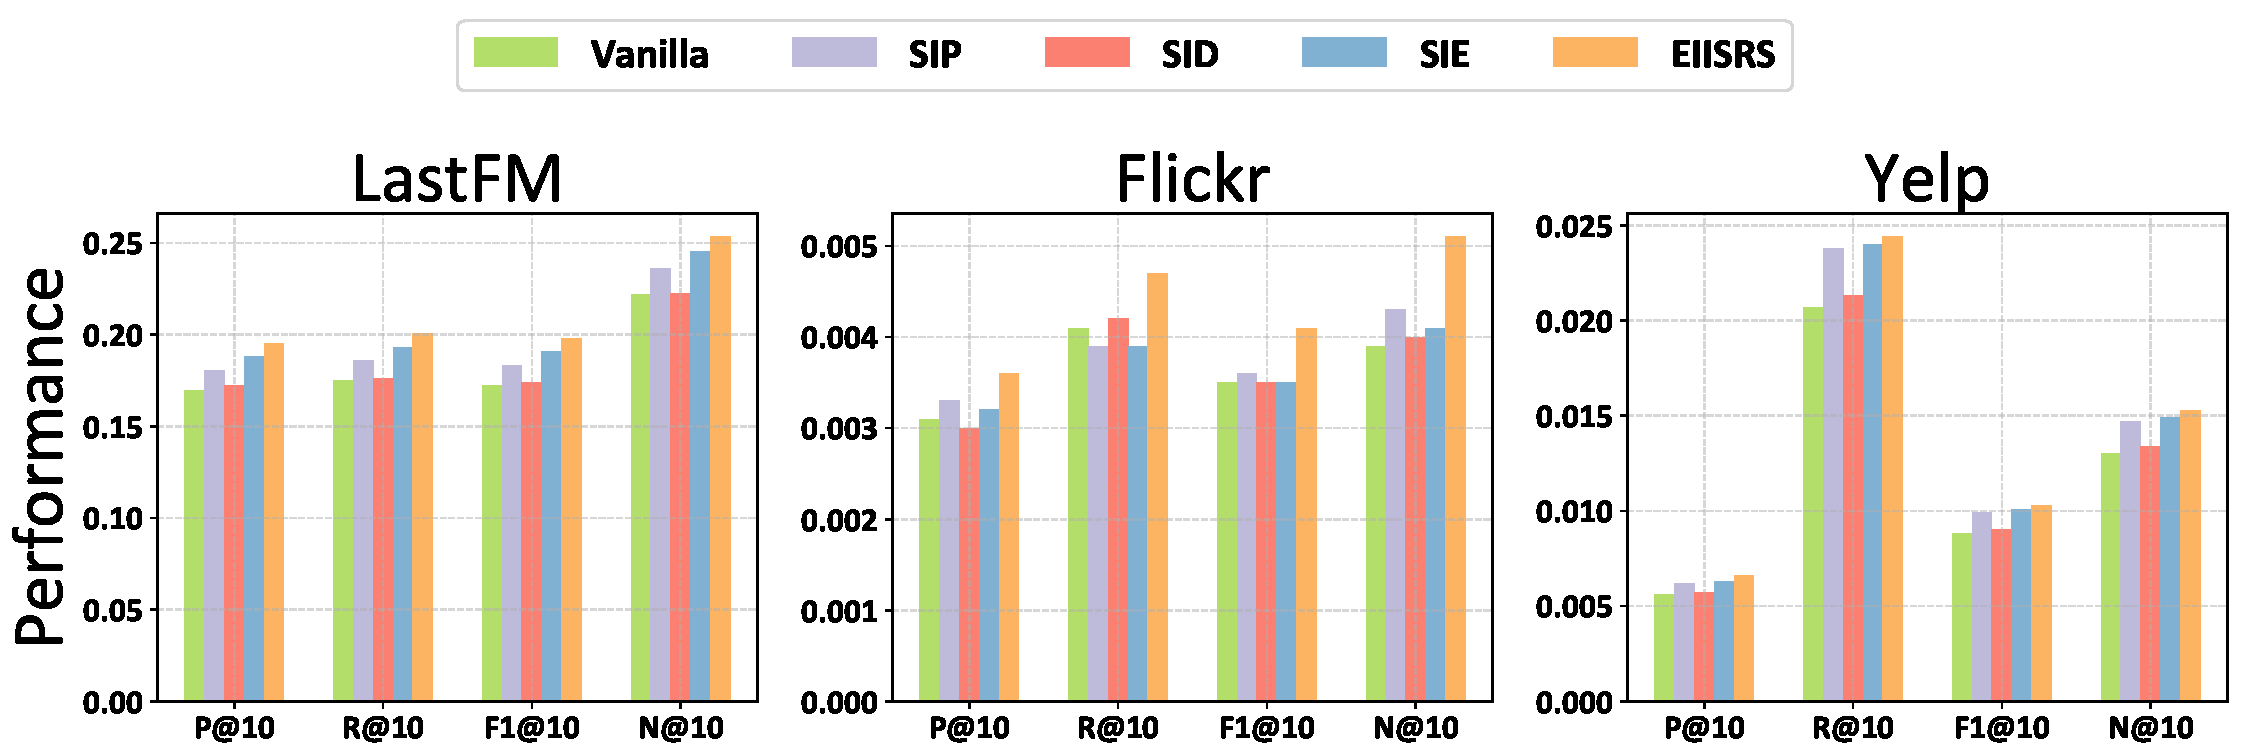
\includegraphics[width=0.45\textwidth]{ablation.pdf} %1.png是图片文件的相对路径
  \caption{Ablation study on different components.}
  \label{fig_ablation}
\end{figure}
% We want to investigate the effectiveness of each component in the first place. We set up four variants by removing certain parts of EIISRS for comparison with our original complete model (i.e., EIISRS). SIP, SID, and SIE refer to the variants that have removed the Social Influence Propagation, Social Influence Diversity, and Social Influence Exploration, respectively. Vanilla is the backbone that is rid of all three components. According to Figure \ref{fig_ablation}, we can easily observe that performances have deteriorated after removing any components. The most significant decrease happens in SID. We are convinced that simulation of social influence diversity can better handle the sparsity and inconsistency problem from social networks for social recommendations. Compared with Vanilla, we can also conclude that each component makes a difference to our model. And the corporation of them matters as well.
To investigate the effectiveness of each component in the model, we create four variants by removing certain parts of EIISRS, and we compare them with our original complete model (i.e., EIISRS). SIP, SID, and SIE refer to the variants where Social Influence Propagation, Social Influence Diversity, and Social Influence Exploration have been removed from the model, respectively. Vanilla refers to the backbone model, which has removed all three components. From Figure \ref{fig_ablation}, we can easily observe that the performance becomes worse after removing any components. The most significant performance drop happens in SID. Therefore, we are convinced that the simulation of social influence diversity is well-suited to tackle the sparsity and inconsistency issue on the social network for social recommendations. Meanwhile, by comparing with Vanilla, we conclude that every component is contributing to our model, and the corporations between components matter as well.
\begin{figure}[ht!]
  \centering
  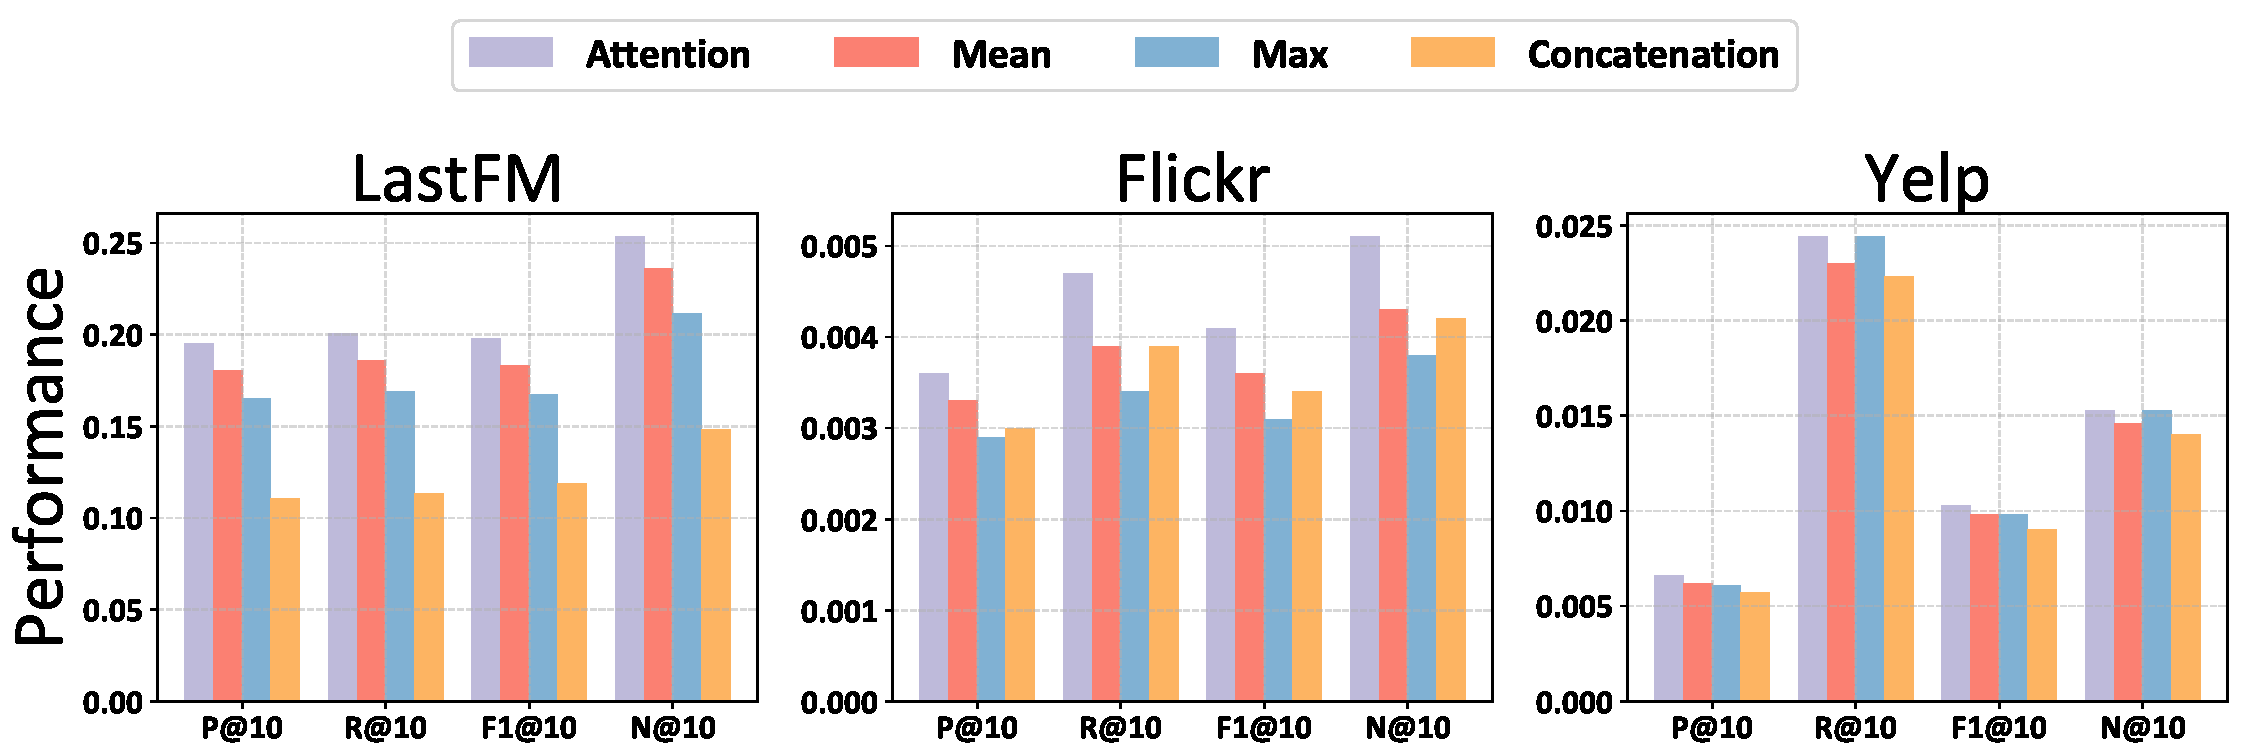
\includegraphics[width=0.45\textwidth]{agg.pdf} %1.png是图片文件的相对路径
  \caption{Ablation study on aggregation methods.}
  \label{fig_agg}
\end{figure}

% In LightGCN, the authors have demonstrated that the weighted sum of different layers in their model is redundant. We set up another ablation study on the aggregation methods to discover their validity in our model. As shown in Figure \ref{fig_agg}, we may find that Attention-based aggregation outperforms any other aggregation methods, such as Mean pooling, Max pooling, and Concatenation. The reasons can be derived from (1) attentive weights can well reflect the social influence propagation, while it would cease on item perspectives among bipartite graph; (2) aggregation is followed with the simulation of social influence diversity, which boosts the distinguishability and accessibility of social information from different scopes of neighborhoods. We also find out that the follow-up methods vary from datasets. 
In LightGCN, the authors demonstrated that the weighted sum of different layers is redundant in their model. To verify the validity of layerwise attention in our case, we set up another ablation study on the aggregation methods. As shown in Figure \ref{fig_agg}, we may find that Attention-based aggregation outperforms any other aggregation methods, including Mean pooling, Max pooling, and Concatenation. The reasons are as follows: (1) in the LightGCN case, layerwise attention is ineffective due to the user-item alternation on the bipartite graph, but in our case, it can well capture the patterns of social influence propagation on the social graph; (2) by combing the attentive aggregation with social influence diversity, the social information from different scopes of neighborhoods can be further generalized and disentangled.

\subsubsection{Hyperparamter Analysis.}
% As for the number of generated implicit neighbors, we can observe that the performance of our model would reach the peak when the number of new neighbors is 30 (in Figure \ref{fig_hyper}). Generally speaking, the decrease in performance is much smaller if we compare it with ESRF \cite{ESRF}. Moreover, even when the number of neighbors becomes large enough, the curve fluctuates in a small range, meaning the sensitivity of the hyperparameter has been alleviated. And the model still works better than most other representative models. It states the effectiveness of the Bernoulli Sampling to deal with the degradation as the number of candidate neighbors increases.
Figure \ref{fig_hyper} shows the model performance with different numbers of generated implicit neighbors. We observe that the model performance reaches its peak when there are 30 new neighbors. Moreover, even when the number of neighbors becomes large enough, the curve fluctuates only within a small range, and the model still outperforms most other representative models. This reflects that the common over-sensitivity issue of the hyperparameter has been well alleviated, which is attributed to the effectiveness of the Bernoulli Sampling in our model, such that the social network structure is not damaged even with a large number of candidate neighbors.
\begin{figure}[ht!]
  \centering
  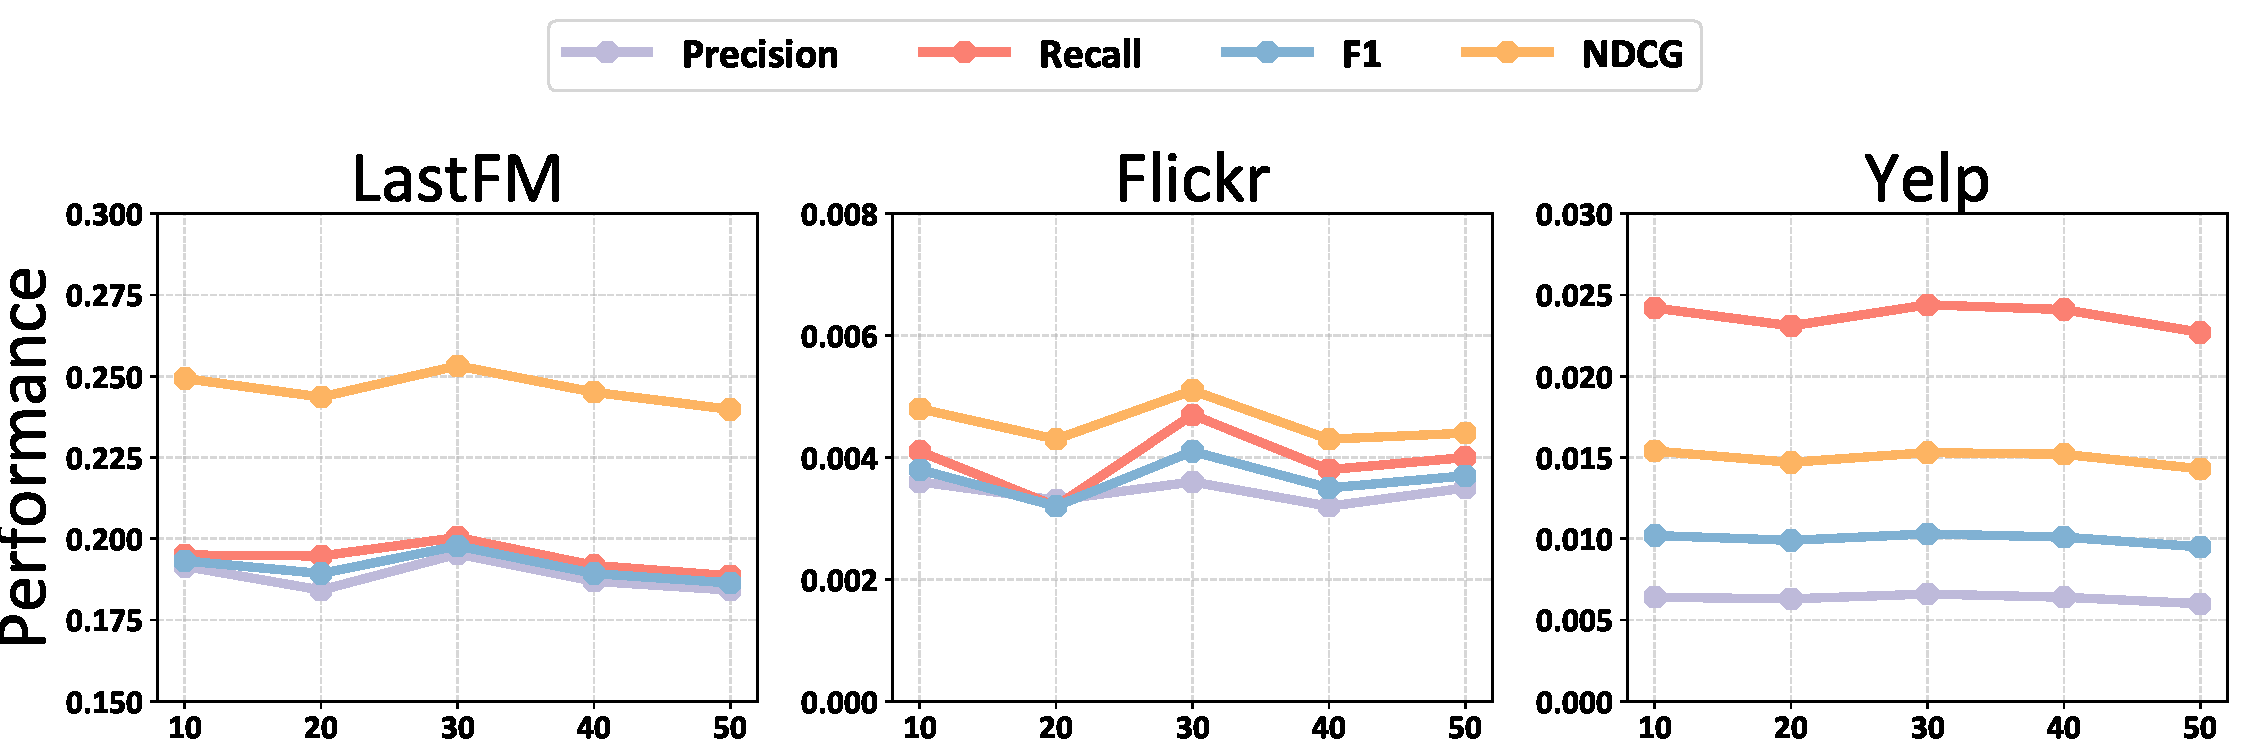
\includegraphics[width=0.45\textwidth]{hyper.pdf} %1.png是图片文件的相对路径
  \caption{The influence of the number of generated implicit neighbors.}
  \label{fig_hyper}
\end{figure}

\section{Related Works}
Social recommendation comes across its blossom with the development of GNN \cite{GCN, MPNN, graphsage} and contrastive learning \cite{sgl}, since the former simulates the social influence and the latter well disentangles social relations. Hence, graph-based recommenders \cite{ngcf,lightgcn} spring up. Since contrastive learning is self-supervised as an auxiliary task and its mechanism still remains unclear\cite{augmentation}, we neglect it so far and put it into future work. Besides, inspired by attention mechanism \cite{attention} and GAT \cite{GAT}, attentive recommenders \cite{diffnet++} become prevailing, which is used to capture the attention signals from node-wise neighbor users and items. On the other hand, VAE-based recommenders \cite{multivae,jova} show their capability to generate latent representation and reconstruct predictions. As a combination of VAE and graph-based learning, VGAE \cite{VGAE} has high potential in graph-based recommendation \cite{vgae_rec}. Furthermore, instead of harnessing the pairwise graph structure, latest works \cite{MHCN, ESRF} also put views on hypergraphs where multiple connected nodes are attributed with a hyperedge (e.g., Motifs \cite{motif}) since it is believed that hyperedges contain complex high-order connective information. But the sparsity is exacerbated and user representation collapse problem also occurs owing to their insufficiency of comprehensive interests \cite{collapse}.

\section{Conclusion}
%The social recommendation system gains more and more attention with the rapid development of social media and big data processing. However, few recent works shift the perspective from taking it the same as the bipartite graph towards considering it as raw data that needed to be processed in the meantime. 
% In our work, we develop a novel recommendation model that mainly focuses on tackling the incompatibility problem inherent in the social network. We learn the layerwise representations of neighborhoods and design LEG-VAE to simulate the social influence diversity. Then, we apply a layerwise graph attention network to capture the propagation of social influence. Finally, we propose a dual sampling method to explore implicit social neighbors. The innovation of using both samplings in our work can better settle the representation collapse problem that happened to sparse users. Extensive empirical studies give solid evidence showing our model is feasible, efficient, convincible, and agile in design.
In our work, we develop a novel recommendation model that mainly focuses on tackling the incompatibility problem inherent in the social network. We learn the layerwise representations of neighborhoods on the social graph and design LEG-VAE to simulate the social influence diversity. Then, we apply a layerwise graph attention network to capture the propagation of social influence. Finally, we propose a new dual sampling method to explore implicit social neighbors. With dual sampling, the representation collapse problem caused by user sparsity can be well addressed. Extensive empirical studies provide solid evidence that our model is feasible, efficient, and agile in design.

\bibliography{aaai24}
\end{document}
